\section{Vertex Locator (VELO)}
\label{section: velo}
%=========================================================================%
%=============================  Vertex reconstruction  ==========================%
%=========================================================================%
%The properties of these decays such as the decay position, lifetime of the B/D mesons and their  products need also to be highly accurate in order to minimise the uncertainty on the key measurements at the LHCb experiment.  
%Particle interactions are characterised by particles originating from a common point in space. With the presence of interacting particles In the case of particle production or with the association of a single parent particle in interactions involving decays.
%
%Since the focus of the LHCb experiment is the observation of rare decays it follows that the detector be optimised such that 
%
%The position of beam proton-proton interactions and particle decays are described by a vertex. A vertex provides information on the position of the event and the particles produced as a result. The identification, positional accuracy of vertices along with the correct association of interactions to their product particles is fundamental in achieving the physics goals of the LHCb experiment, its presence in an event serves as a clear indicator of the rare physics processes that are the focus of the LHCb detector. 
%
%Unique to the LHCb detector.
%
%Vertex reconstruction of interaction points and decay vertices is an extremely important aspect of the LHCb experiment. This is due to the primary focus of the experiment being around the analysis of rare decay processes. From this is follows that the LHCb detector must have good tracking around the interaction region such that a vertex which has been inferred from the direction of the tracks has a small error on its position and i.e. decay lifetime. In addition to this accurate tracking is required in order to accurately measure the impact parameter of tracks, an important input for the trigger.

%Particle interactions are characterised by particles originating from a common point in space. With the presence of interacting particles In the case of particle production or with the association of a single parent particle in interactions involving decays.
%
%Since the focus of the LHCb experiment is the observation of rare decays it follows that the detector be optimised such that 
%
%The position of beam proton-proton interactions and particle decays are described by a vertex. A vertex provides information on the position of the event and the particles produced as a result. The identification, positional accuracy of vertices along with the correct association of interactions to their product particles is fundamental in achieving the physics goals of the LHCb experiment, its presence in an event serves as a clear indicator of the rare physics processes that are the focus of the LHCb detector. 
%
%Unique to the LHCb detector.
%
%Vertex reconstruction of interaction points and decay vertices is an extremely important aspect of the LHCb experiment. This is due to the primary focus of the experiment being around the analysis of rare decay processes. From this is follows that the LHCb detector must have good tracking around the interaction region such that a vertex which has been inferred from the direction of the tracks has a small error on its position and i.e. decay lifetime. In addition to this accurate tracking is required in order to accurately measure the impact parameter of tracks, an important input for the trigger.
%To achieve this the LHCb detector has a dedicated vertex reconstruction sub-detector called the VELO detector. The VELO detector is made up of a series of silicon stations which are positioned along the direction of the beam (Fig \ref{fig: VELO_silicon_stations}). Each station is segmented into two halves such that the two halves of the VELO can through a mechanical system move into open and closed configurations(Fig \ref{fig: VELO layout}).
%
%This mechanism enables the VELO detector to maximise its resolution by minimising the distance between the nominal interaction region and the sensitive areas of the VELO. During periods of stable beam the minimum distance between the nominal interaction region and the sensitive area of the VELO detector is $ \approx 5mm$. However during the process of beam injection the width of the beam can be greater. To protect the components of the VELO during this process the two halves of the VELO are separated by as much as $6mm$.

%\begin{itemize}
%	\item Station layout
%	\item r-$\phi$ sensors
%	\item pile-up sensors and L0 trigger
%	\item LHC vacuum and VELO vacuum
%	\item RF foils
%\end{itemize}

%1. VELO motivation
%2. VELO features and layout
%3. VELO performance

The detection of rare B and D meson decays is a key requirement to meet the physics goals of the LHCb experiment.  In the LHCb detector these processes are characterised by the presence of production and decay vertices. To maximise the sensitivity of detecting and correctly identifying these events via the presence of displaced vertices a dedicated sub-detector system called the VELO (Vertex locator) is employed around the nominal interaction region. The detection of vertices is achieved indirectly via the detection of their decay products through track reconstruction, the paths of which are extrapolated towards a common point of intersection to give the vertex. The reconstruction of VELO tracks is also important for use in the LHCb trigger system, discussed in section \ref{section: trigger}.

The VELO is a silicon micro strip vertex detector, it is made up of two halves (left and right) each containing twenty one track station modules (figure \ref{fig: VELO_silicon_stations}) positioned at different points along the beam axis. The angular coverage of the VELO detector is shown in figure \ref{fig: velo angular acceptance}.

\begin{figure}
	\centering
	\includegraphics[width=0.5\columnwidth]{/Users/admin/Dropbox/LHCb/detector/VELO/images/silicon_stations.jpg}
	\caption{VELO silicon stations during partial construction of the VELO sub-detector}
	\label{fig: VELO_silicon_stations}
\end{figure}

\begin{figure}
	\centering
	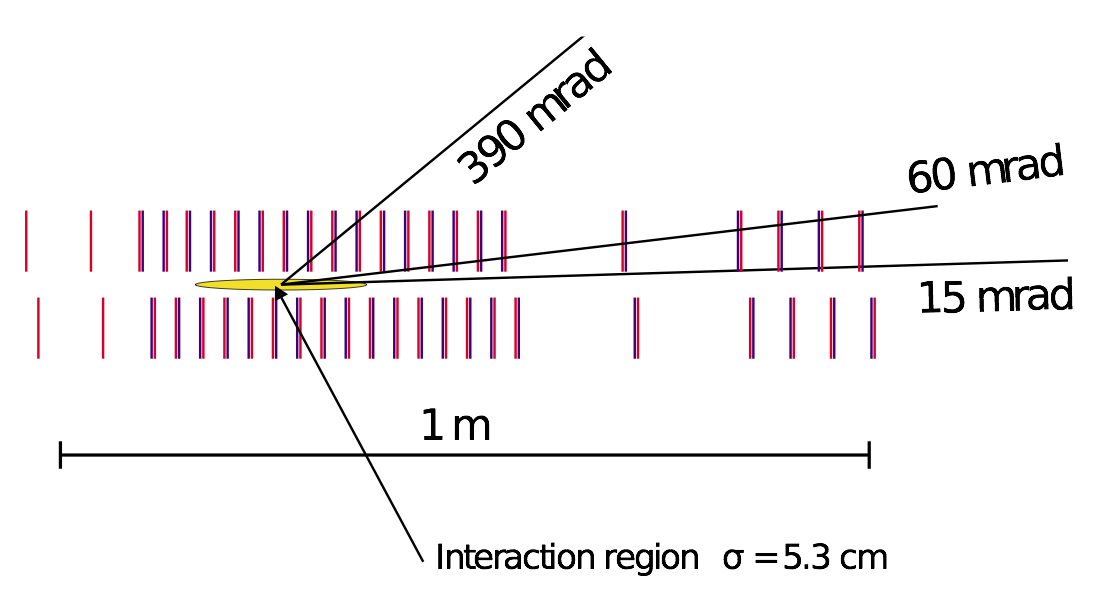
\includegraphics[width=0.7\columnwidth]{Chapters/detector/images/velo_angular_acceptance.png}
	\caption{The layout of the VELO R (red) and $\phi$ (blue) sensors shown in the (x,z) plane. A $\pm2\sigma$ area around the nominal interaction point is shown in yellow. Lines drawn at 390 mrad and 15 mrad represent the maximum and minimum angular coverage, while the line at 60 mrad shows the average track angle in minimum bias events. The left-most two pairs of R sensors are the pileup veto stations.}
	\label{fig: velo angular acceptance}
\end{figure}

Modules are approximately semi-circular in shape, 300 \,$\mu$m thick, with an outer diameter of 84 mm and an inner diameter of 8mm in order to accommodate the beam pipe. Each module is composed of a pair of sensors which measure the radial distance and azimuthal angle of particles traversing the detector. The silicon strips of the radial sensor are orientated radially about the module and in concentric semi-circles for the azimuthal sensor, see figure \ref{fig: r-phi sensors}. The modules are also contained within a secondary vacuum to reduce background contributions from interactions with gas particles in the beam pipe, this is enclosed by a 300$\mu$m thick aluminium foil which also protects from radio frequency pickup from the beam.

\begin{figure}
	\centering
	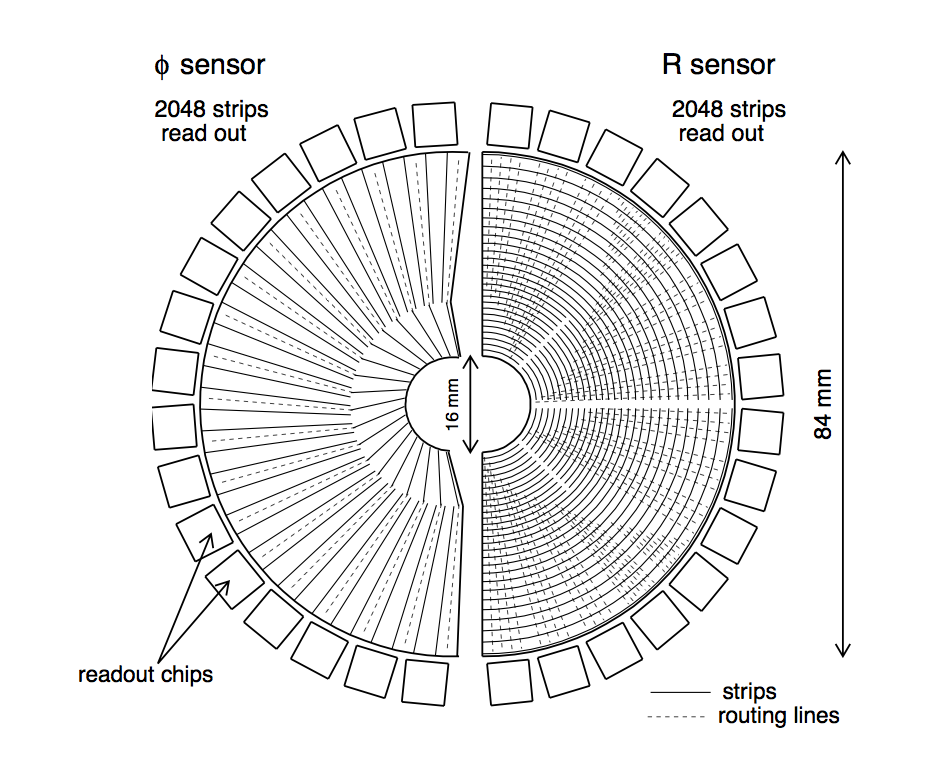
\includegraphics[width=0.5\columnwidth]{Chapters/detector/images/r-phi_sensors.png}
	\caption{Schematic diagram of a VELO station from the perspective of along the beam line. Each half consists of both R and $\phi$ sensors though in this figure only the $\phi$ sensors are shown in the left half and only the R sensors are shown in the right half.}
	\label{fig: r-phi sensors}
\end{figure}

The two halves of the detector open and close about the interaction region depending on the status of the LHC beam (see fig \ref{fig: VELO layout}). During the beam fill or dumping the VELO is put into its open configuration in order to minimise radiation damage to its components. When the beam is stable the VELO is configured into its closed configuration (In this configuration the minimal distance between the silicon trackers and the beamline is 8mm) to maximise its tracking resolution.

\begin{figure}
	\centering
	\includegraphics[width=\columnwidth]{/Users/admin/Dropbox/LHCb/detector/VELO/images/VELO_open_closed.png}
	\caption{The front face of the first modules illustrated in two configurations. Closed (left): Once the beam position is stable the halves close so that the position between the VELO and the interaction region is minimised. Open: The two halves are separated in order to protect the modules from the unstable beam.}
	\label{fig: VELO layout}
\end{figure}

Figure \ref{fig: pv resolution} shows the resolution of the primary vertex position as a function of track multiplicity and figure \ref{fig: ip resolution} shows the resolution of the impact parameter as a function of $p_\mathrm{T}^{-1}$. Both of these measurements approach the expected design parameters \cite{Latham:1491236}.

%The VELO reconstructs vertices with a resolution of $\sim10\,\mu$m; this corresponds to a $\sim40$ fs resolution in the measurement of particle lifetimes and an impact parameter resolution of $20\,\mu$m. %Reconstructs particles from $15$ mrad to $390$ mrad.

\begin{figure}[h]
	\centering
	\begin{subfigure}[b]{0.45\textwidth}
		\includegraphics[width=\columnwidth]{/Users/admin/Dropbox/LHCb/detector/VELO/images/pv_resolution_xy.png}
		\caption{x in red, y in blue}
	\end{subfigure}
	\begin{subfigure}[b]{0.45\textwidth}
		\includegraphics[width=\columnwidth]{/Users/admin/Dropbox/LHCb/detector/VELO/images/pv_resolution_z.png}
		\caption{z}
	\end{subfigure}
	\caption{Resolution of primary vertex position}
	\label{fig: pv resolution}
\end{figure}

\begin{figure}[h]
	\centering
	\includegraphics[width=\columnwidth]{/Users/admin/Dropbox/LHCb/detector/VELO/images/ip_resolution.png}
	\caption{Impact parameter resolution as a function of $p_T^{-1}$}
	\label{fig: ip resolution}
\end{figure}

